Et gyroskop, eller en gyrosensor måler endring i rotasjon langs pitch, roll og yaw aksene. 
I likhet med akselerometer og magnetometer er gyroskop som benyttes i elektronikk bygget på MEMS-teknologi. 
MEMS-gyroskop benytter coriolisakselerasjonen som er en akselerasjon som oppstår på et legeme som 
beveger seg i en rett linje på et roterende referansesystem. Coriolisakselerasjonen vil da oppstå vinkelrett på bevegelsen. \parencite{Gron2021coriolis}
Figur \ref{fig:mems-gyro} viser et eksempel på et MEMS-gyroskop. Det består av en vibrerende struktur som holder en deteksjonsstruktur (grønn). 
Når sensoren er stabil, vil deteksjonsstrukturen bevege seg frem og tilbake med den vibrerende strukturen. 
Ved rotasjon vil deteksjonsstrukturen skyves ut til siden på grunn av coriolisakselerasjonen. 
For å beregne rotasjonen benyttes endringen i kapasitansen mellom kammene i deteksjonsstrukturen som oppstår ved forskyvningen. 

\begin{figure}[htp]
    \centering
    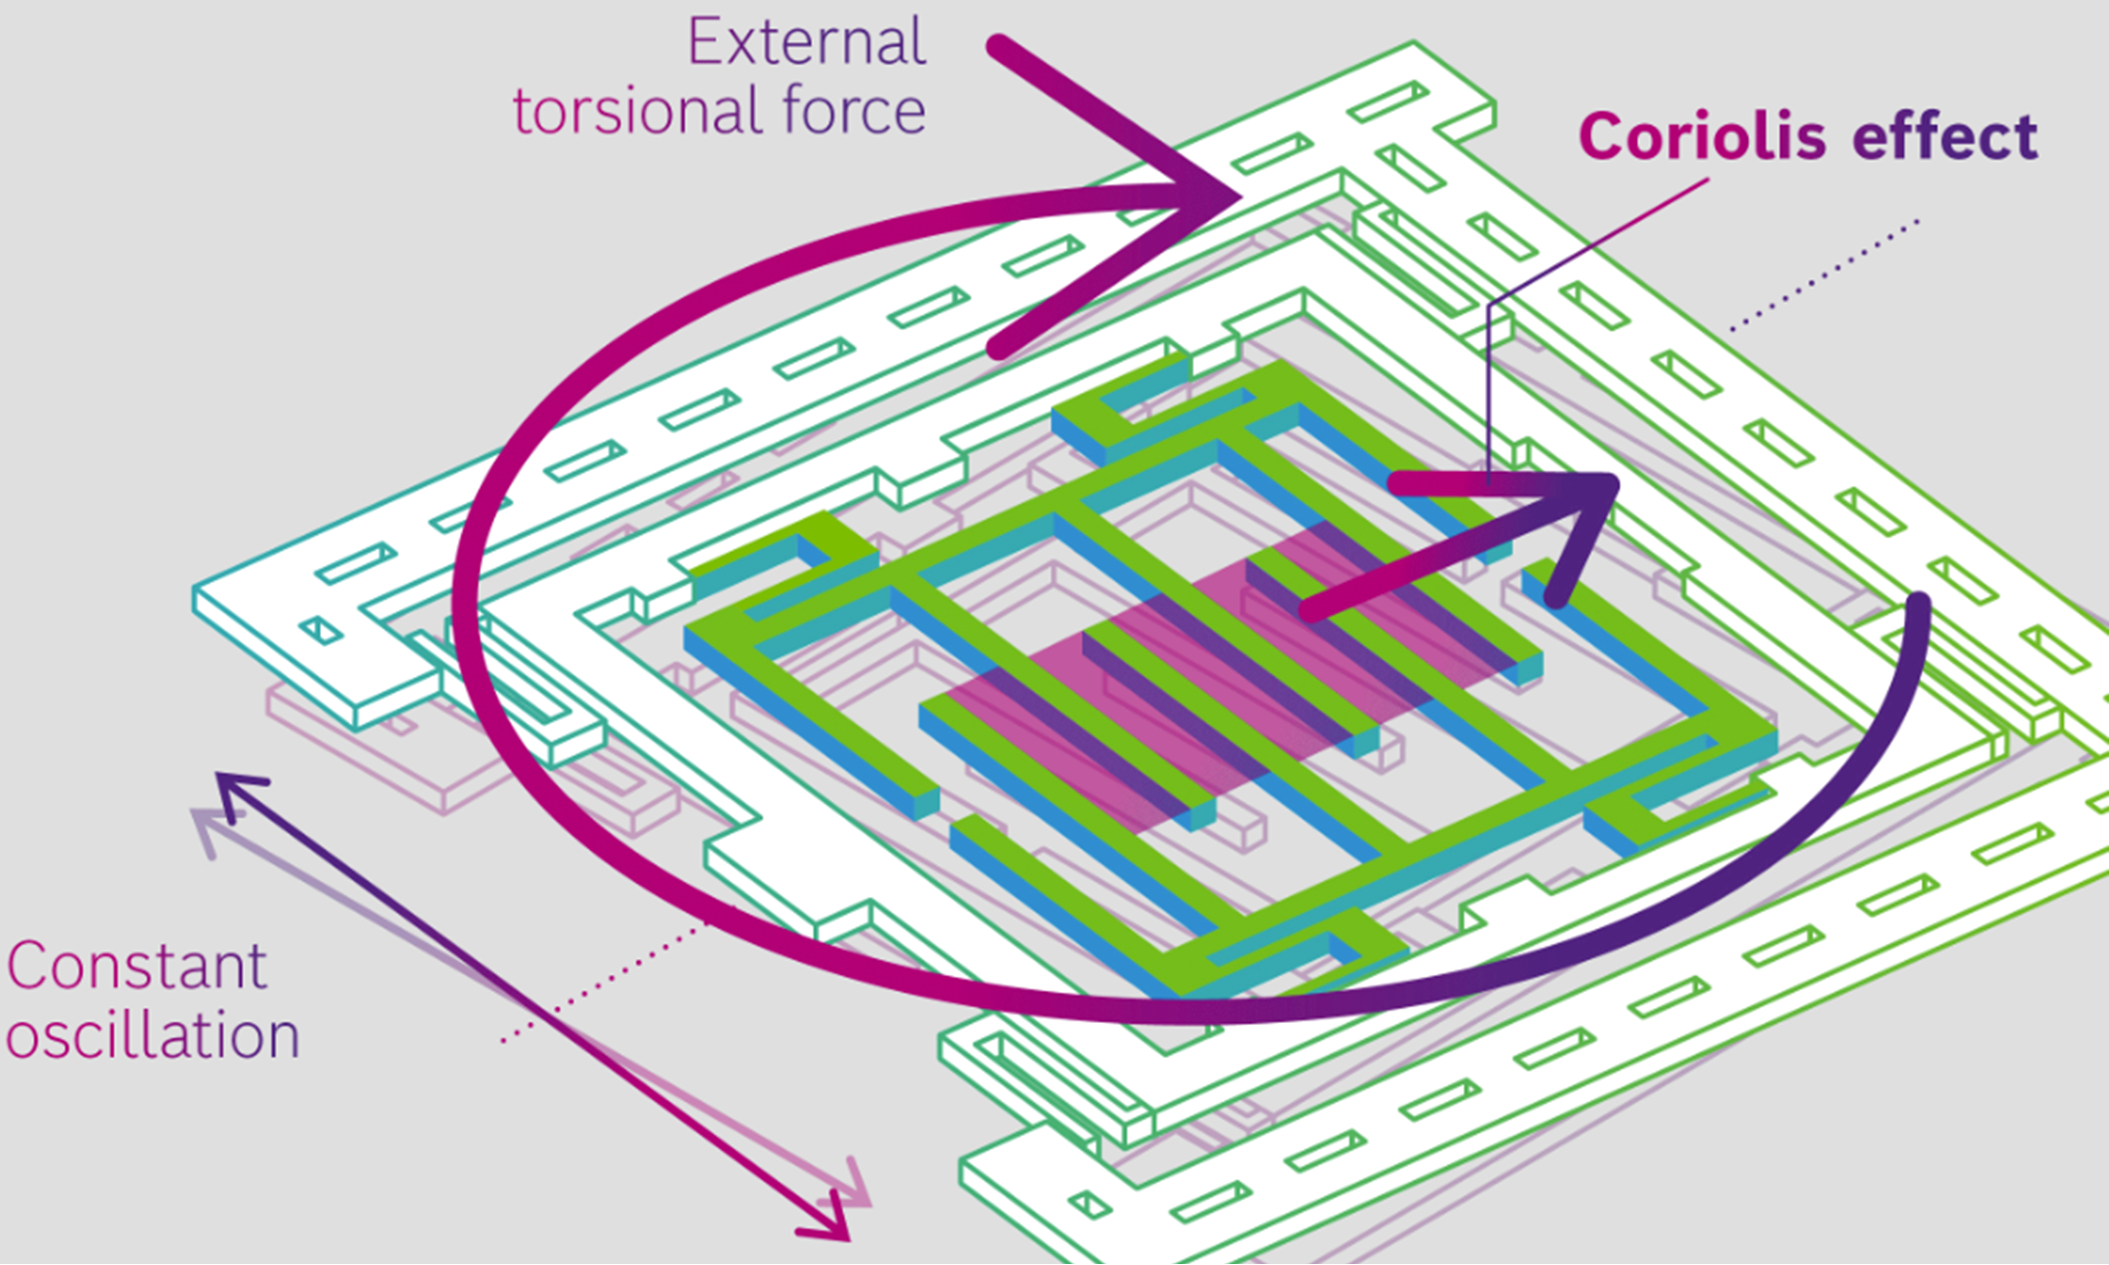
\includegraphics[width=0.5\columnwidth]{figures/mems-gyro}
    \caption{MEMS-gyroskop. \parencite{Bosch}}
    \label{fig:mems-gyro}
\end{figure}

Figur \ref{fig:mems-gyro} viser en enkel rotasjonssensor som kun vil detektere rotasjon rundt 
aksen som står vinkelrett på deteksjonsstrukturen. For å detektere rotasjon i tre akser må 
flere slike rotasjonssensorer med forskjellig orientering kombineres. \parencite{Bosch}
